\chapter{Neutrino Detection}
\label{chap:nu-detection}

Neutrino physics has seen massive progress from first detection \num{60}~years ago to planned billion dollar experiments in the near future.
This chapter will give an overview of the history of neutrino detectors, describe the current state of the field and then introduce the most relevant physics.

\section{History}
In 1914, Chadwick proved that the energy spectrum of the $\beta$-decay was continuous.~\cite{contBeta}
As an explanation for this, Wolfgang Pauli in 1930 proposed a new neutral, weakly interacting fermion to the \emph{Radioactive Ladies and Gentlemen}~\cite{pauliLetter} which he called the \emph{neutron}.
However, the same Chadwick in 1932 discovered the particle we today call neutron.~\cite{neutron}
Upon this, Fermi proposed the name \emph{neutrino} and a little later came up with a new theory for $\beta$-decay.~\cite{betaDecay}

It took almost another quarter of a century until the neutrino was experimentally detected for the first time by Reines and Cowan in 1956.~\cite{reinesCowan}
They built a detector for the reaction
\begin{IEEEeqnarray}{rCl}
	\label{eq:nu-detection_reinesCowan}
	\nueb + p & \rightarrow & e^+ + n
\end{IEEEeqnarray}
and put it next to the nuclear reactor of the Savannah River Plant in South Carolina, US.
It consisted of two water tanks sandwiched in between three liquid scintillator tanks with photomultiplier tubes (PMTs) on the sidewalls.
The water was the target to induce the above reaction while the scintillator tanks had the task of detecting the resulting positron and neutron.
A free positron slows down in matter and eventually gets captured by a shell electron which produces two back-to-back $\gamma$s with an energy of \SI{511}{\kilo\electronvolt} each.
These produce scintillation light in the two adjacent tanks and thus can be detected by forming a coincidence of the PMTs of the two tanks.
Neutron detection is achieved by doping the water target with cadmium which captures the free neutrons producing multiple $\gamma$s that can again be detected using the coincidence of the two adjacent scintillator tanks.
The neutron capture is much slower than the positron one.
Therefore, the process from Equation~\eqref{eq:nu-detection_reinesCowan} produces a very distinct signal in the detector consisting of a pulse with a lower amplitude from the positron capture and another one with a higher amplitude from the neutron capture a few \si{\micro\second} later.
Backgrounds can be efficiently rejected employing this technique.
That drawback is that detection is limited to the \nueb{} interaction in Equation~\eqref{eq:nu-detection_reinesCowan}.

In 1962, Lederman et al.\ proved the existence of the \numu{} at the Alternating Gradient Synchrotron (AGS) at Brookhaven National Laboratory (BNL) in New York, US.~\cite{numu}
For the first time, they produced \numu{}s using an accelerator.
The protons from the AGS were guided onto a beryllium target producing pions which in turn decay according to
\begin{IEEEeqnarray}{rCl}
	\label{eq:nu-detection_pion-decay}
	\pi^+ & \rightarrow & \mu^+ + \numub \\
	\pi^- & \rightarrow & \mu^- + \numu
\end{IEEEeqnarray}
producing a beam of muon (anti)neutrinos.
\emph{Spark chambers} were used to detect the neutrinos.
They were placed behind a \SI{13.5}{\metre} wall of iron shielding used to stop the muons and remaining hadrons from the beam.

A spark chamber consists of several parallel conducting plates immersed in a counting gas, typically a mixture of helium and neon.
Every other plate is connected to a pulsed high-voltage power supply while the rest is grounded.
At either end of the stack, triggering detectors (usually scintillators coupled to PMTs) are placed.
When two coinciding signals from these are received, a high-voltage pulse is applied to the plates.
If this happens fast enough ($\order{\SI{10}{\micro\second}}$), a spark forms along the electric field lines where the counting gas has been ionised by the incident particle(s).
The amplitude and the duration of the HV pulse need to be carefully tuned in order to reach the threshold of spark formation but to prevent random sparks on sharp edges and spacers etc.
A gas amplification of \numrange{e8}{e9} is required to achieve this.
Furthermore, the rising edge of the HV pulse needs to be extremely short ($\order{\SI{1}{\nano\second}}$).
If it was too long, it would drift the ionised track towards the electrodes before the field is high enough to initiate a discharge.
Switching high voltages at this speed is not easy.
Additionally, spark chambers have quite high dead times of $\order{\SI{100}{\milli\second}}$ which is needed for the ionisation charge to clear.
A \emph{clearing field} or an electronegative quenching gas additive can be used to speed up this process.~\cite{grupen}

In the 1960's, after Davis failed to measure the lepton-number-violating reaction
\begin{IEEEeqnarray}{rCl}
	\label{eq:nu-detection_homestake}
	\nueb + \ce{^{37}Cl} & \rightarrow & \ce{^{37}Ar} + e^- \m{,}
\end{IEEEeqnarray}
he decided to replace the \nueb{} by solar \nue{}.~\cite{homestake68, homestake98}
Surprisingly, they measured a flux approximately on third lower than predicted by the standard solar model (SSM).
This result became famous as the solar neutrino problem only to be resolved more than \num{30} years later by the SNO experiment.
Davis' experiment was located \SI{1478}{\metre} (\SI{4200}{\metre} water equivalent) underground in the Homestake gold mine at Lead, South Dakota, US.
The detector consisted of a tank filled with \SI{615}{\tonne} of tetrachloroethylene, \ce{C_2Cl_4}.
As opposed to the two experiments above, this was a \emph{radiochemical} detector which can only detect neutrino interactions offline.
According to Equation~\eqref{eq:nu-detection_homestake}, an incident neutrino converts one of the chlorine atoms in the detector into an unstable argon isotope.
After exposure, the tank is purged by pumping helium gas through the liquid which extracts the argon isotopes.
In order for this to work, a certain amount of \ce{^{36}Ar} is introduced into the tank as a carrier.
Through a sophisticated system, the argon is purified and finally, its \ce{^{37}Ar} content is measured in a \emph{proportional counter}.
By counting the number of decaying argon isotopes and extrapolating using its half-life of \num{35} days, it is possible to calculate the number of neutrino interactions during the exposure.

A proportional counter is a container with two electrodes (usually a cylinder with a wire in its centre) filled with a counting medium (usually gaseous).
Incident charged particles ionise the counting medium---neutral particles can be detected if they first produce charged particles via interaction with matter in or surrounding the detector.
If an electric field is applied to the electrodes, the produced electron-ion pairs are separated and drift towards the corresponding electrode.
By reading out the current on the electrodes, one can measure the amount of ionisation produced inside the detector.
Usually, the anode is read out because the drift velocity of electrons in an electric field is much higher than the one of ions.
In this regime, the detector is in fact an ionisation counter rather than a proportional counter.
The problem is that the charge produced by the ionisation is very low and the current detector needs to be very sensitive.
By increasing the voltage across the electrodes, the sensitivity can be improved.
If the field inside the counter is above a certain threshold, the drifting ionisation electrons become energetic enough to ionise the counting medium themselves and thus, start an avalanche and produce more charge.
In the appropriate voltage range, the produced charge is still proportional to the primary ionisation charge, thus the name proportional counter.
The voltage can be raised further to enter the Geiger regime where the avalanches produce UV photons in addition to the ionisation.
These UV photons travel independently of the electric field and can start new avalanches via the photoelectric effect.
The process can only be stopped by quenching the discharge either electrically (temporary voltage reduction) or chemically (quenching additive).

While the Homestake experiment provided a clean way of counting \nue{} interactions, it provided no information on the timing, direction and kinematics of the interaction.
Only a lower energy threshold is given by the fact, that the neutrino needs to have enough energy to dissociate the chlorine atom from the tetrachloroethylene molecule.
Due to this, it was not possible to tell which reaction chain in the sun, the detected neutrinos originated from.
Furthermore, care needs to be taken for a very good understanding of all background processes that can produce \ce{^{37}Ar} or its signature in the counting tube.
Finally, this experiment was only capable of detecting \nue{} which proved to be crucial in the solution to the solar neutrino problem; oscillation.

In 1988, the Kamioka Nucleon Decay Experiment (KamiokaNDE), in the Kamkioka mine in Japan, and the Irvine-Michigan-Brookhaven (IMB) detector found a similar deficiency in atmospheric neutrinos which actually were a background for the original experiments looking for proton decays.\todo{find source for IMB or remove}
Atmospheric neutrinos are produced in a similar fashion than Lederman et al.\ did in their muon neutrino beam experiment.
Cosmic rays strike the Earth atmosphere and produce secondary particles many of which are pions, in turn, decaying according to Equation~\eqref{eq:nu-detection_pion-decay}.
Thus, atmospheric neutrinos are mainly \numu{}/\numub{}.
However, the muon neutrino flux measured by KamiokaNDE was only \SI{59+-7}{\percent} of the one predicted by Monte Carlo simulations.~\cite{kamiokandeAtmos}
After an upgrade (Kamiokande II), the collaboration furthermore confirmed the solar neutrino problem discovered by the Homestake experiment.~\cite{kamiokandeSolar}
The detector was a \SI{3000}{\tonne} water tank equipped with \num{1000} PMTs to detect \emph{Cherenkov} radiation produced by incoming charged particles.

Upon passage of a charge particle, the atoms of the medium become electric dipoles by means of polarisation.
If the velocity of the incident particle $v$ is greater than the the speed of light inside the medium $\frac{c}{n}$, defined by the refractive index $n$, this polarisation is not symmetric anymore, resulting in a non-vanishing dipole moment.
A characterisitic cone-shaped radiation in the direction of the particle is the result.
The half opening angle of the cone is given by
\begin{IEEEeqnarray}{rCl}
	\cos(\theta_{\m{c}}) & = & \frac{c}{n \qty(\lambda) v}
\end{IEEEeqnarray}
and the radiation spectrum is
\begin{IEEEeqnarray}{rCl}
	\dv{N}{x} & = & 2 \pi \alpha z ^ 2 \int_{\lambda_1}^{\lambda_2} \qty(\frac{\sin(\theta_{\m{c}} \qty(\lambda))}{\lambda}) ^ 2 \dd{\lambda}
\end{IEEEeqnarray}
with the number of Cherenkov photons $N$, path length $x$, fine-structure constant $\alpha$, and electric charge of the particle $z$.
By recording the ring produced by this cone with light detectors, it is possible to determine the timing, direction, momentum and type of the incident charged particle within certain restrictions.
Often employed detection media include water and oil while the photodetectors are usually PMTs.~\cite{grupen}

The charged particles detectable by a Cherenkov detector can be produced by neutrinos in multiple ways.
Here, only the two most important processes shall be introduced, a more detailed description will be given in Section~\ref{sec:nu-detection_interactions}.
Analogously to Equation~\eqref{eq:nu-detection_reinesCowan}, neutrinos of all three flavours can interact with nucleons according to
\begin{IEEEeqnarray}{rCl}
	\label{eq:nu-detection_CC-nu}
	\nu_l + n &				\rightarrow &	l^- + p \\
	\label{eq:nu-detection_CC-antinu}
	\nub_l + p &	\rightarrow &	l^+ + n
\end{IEEEeqnarray}
with $l = e,\mu,\tau$.
It should be noted however, that usually $\tau$ leptons are too short-lived to produce enough Cherenkov radiation to be detected.
A second interaction path of neutrinos with matter is the scattering off shell electrons according to
\begin{IEEEeqnarray}{rCl}
	\label{eq:nu-detection_NC-nu}
	\nu_l + e^- & \rightarrow & \nu_l + e^- \\
	\label{eq:nu-detection_NC-antinu}
	\nub_l + e^- & \rightarrow & \nub_l + e^- \, \m{.}
\end{IEEEeqnarray}
If the neutrino momentum is high enough, the electron recoil can be detected by a Cherenkov detector for all three flavours.

While registering timing and directionality in addition to being able to detect and distinguish \nue{} and \numu{} was a huge improvement over the radiochemical Homestake experiment, Cherenkov detectors still suffer from some difficiencies in particle identification.
One of them is that they can only detect charged particles with sufficient momentum to produce Cherenkov radiation rather than detecting the whole event topology.
The detector cannot distinguish between processes producing the same ring signature.
An important example is a $\pi^{\m{0}}$ produced by a \numu{} which produces a signal in a Cherenkov detector very similar to the one of a \nue{}.
This is a crucial background for neutrino oscillation experiments.

Super-Kamiokande, the \SI{50}{\kilo\tonne} successor of Kamiokande, solved the atmospheric neutrino problem in 1998.~\cite{superKAtmos1, superKAtmos2}
It measured the flavour ratio of the atmospheric neutrino flux as a function of the zenith angle.
The ratio of the number of upward to downward $\mu$-like events was found to be $\approx\SI{50}{\percent}$ while from Monte Carlo simulations it was expected to be $\approx\SI{100}{\percent}$.
This result suggested a dissappearance of \numu{} via neutrino oscillations for atmospheric neutrinos that travelled along the much longer baseline through the Earth.

The solar neutrino problem was solved in 2002 by the Sudbury Neutrino Observatory (SNO) in the INCO, Ltd.\ Creighton mine near Sudbury, Ontario, Canada.~\cite{snoSolar}
SNO is a \SI{1}{\kilo\tonne} heavy water Cherenkov detector located \SI{2039}{\metre} below the Earth surface ($\approx\SI{6000}{\metre}$ water equivalent).
Its use of heavy water (\ce{D_2O}) allows it to detect neutrinos flavour-independently via
\begin{IEEEeqnarray}{rCl}
	\label{eq:nu-detection_NCsno-nu}
	\nu_l + d & \rightarrow & \nu_l + p + n \\
	\label{eq:nu-detection_NCsno-antinu}
	\nub_l + d & \rightarrow & \nub_l + p + n
\end{IEEEeqnarray}
in addition to the interaction channels detectable by light water Cherenkov detectors given by Equations \eqref{eq:nu-detection_CC-nu}, \eqref{eq:nu-detection_CC-antinu}, \eqref{eq:nu-detection_NC-nu}, and \eqref{eq:nu-detection_NC-antinu}.
For this to work, the emerging neutron needs to be detected which was achieved using \ce{^3He}-filled proportional counters inside the heavy water tank.
The additional neutrino detection channel allowed SNO to prove that only the solar \nue{} flux is below the predictions by the SSM while the combined flux of all three flavours is consistent with the model, providing another strong evidence for neutrino oscillation.

The \nut{} was first detected by the DONUT experiment at Fermi National Accelerator Laboratory (FNAL) near Batavia, Illinois, US, in 2001.~\cite{donut}
Similarly to the \numu{} discovery, a neutrino beam was produced by shooting \SI{800}{\giga\electronvolt} protons from the Tevatron onto a tungsten beam dump.
The \nut{} were detected via the interactions described by Equations~\eqref{eq:nu-detection_CC-nu} and~\eqref{eq:nu-detection_CC-antinu} for $l = \tau$.
Therefore, it was required to detect very short-lived $\tau$ requiring a detector with a very good spatial resolution.

\emph{Nuclear emulsions} were chosen as the core component of the detector.
They consist of fine-grained silver-halide crystals (\ce{AgBr} and/or \ce{AgCl}) embedded in a gelatine substrate.
Ionisation by passing charged particles causes some of the silver-halide molecules to be reduced to metallic silver.
A subsequent development process reduces the silver-halide crystals, preferentially affecting those microcrystals already disturbed and partly reduced by the ionisation.
Finally, the remaining crystals are dissolved in the fixation process leaving a stable image of elemental silver particles along the ionisation tracks.
These charge images can be digitised using Charge-Coupled Device (CCD) cameras attached to computer controlled microscopes.
GPU-accelerated pattern regnition can be employed for event reconstruction.~\cite{grupen}

The spatial resolution of the emulsion is limited by the size of the crystals.
On the other hand, they need to have a certain size in order for ionising particles to be able to reduce enough silver-halide molecules to create a track inside the emulsion.
A compromise needs to be found based on the experimental requirements.
The price for the high spatial resolution is that emulsions are an offline detector that cannot be triggered or vetoed.
An external tracking detector (scintillating fibres in the case of DONUT) are required to record event timing.
Its data needs to be matched to the emulsion data before the actual analysis.

Nowadays, the concept of neutrino oscillation is well established and characterised by Daya~Bay~\cite{dayabayRecent}, T2K~\cite{t2kOsc}, KamLAND~\cite{kamland}, SNO, Super-Kamiokande and many other experiments.
Daya Bay and KamLAND essentially employ the same technique as Reines and Cowan to look for disappearance of nuclear reactor \nueb{}.
The only difference being that instead of using multiple scintillator tanks in coincidence, they use one big tank shielded and vetoed by water and/or mineral oil Cherenkov detectors.
Tokai to Kamioka (T2K) directs a \numu{} beam similar to the one of Lederman et al.\ towards Super-Kamiokande to look for \numu{} disappearance and \nue{} appearance over a long baseline.


\section{Current Status and Future Experiments}
\label{sec:nu-detection_future-exp}

\todo[inline, color=red]{current status and future experiments}


\section{Neutrino Interaction with Matter}
\label{sec:nu-detection_interactions}

\todo[inline]{xsec plot}

\begin{table}[htb]
	\centering
	\caption{Estimated number of interactions per tonne of \ce{Ar} at the \dune{} near detector for approximately one month (\num{1e20} protons on target) exposure to an (anti)neutrino beam produced from a primary proton beam of \SI{120}{\giga\electronvolt} and \SI{1.2}{\mega\watt}.}
	\label{tab:nu-detection_nd-rates}
	\begin{tabu} to \textwidth {|X|S|S|}
		\hline
		Production mode &																						{\numu{} beam} &	{\numub{} beam} \\
		\hline
		\hline
		CC QE ($\numu n \rightarrow \mu^- p$) &																	30000 &				13000 \\
		\hline
		NC elastic ($\numu N \rightarrow \numu N$) & 															11000 &				6700 \\
		\hline
		CC resonant ($\numu p \rightarrow \mu^- p \pi^+$) &														21000 &				0 \\
		\hline
		CC resonant ($\numu n \rightarrow \mu^- n \pi^+ \, (p \pi^0)$) &										23000 &				0 \\
		\hline
		CC resonant ($\numub p \rightarrow \mu^+ p \pi^- \, (n \pi^0)$) &										0 &					8300 \\
		\hline
		CC resonant ($\numub n \rightarrow \mu^+ n \pi^-$) &													0 &					12000 \\
		\hline
		NC resonant ($\numu p \rightarrow \numu p \pi^0 \, (n \pi^+)$) &										7000 &				0 \\
		\hline
		NC resonant ($\numu n \rightarrow \numu n \pi^+ \, (p \pi^0)$) &										9000 &				0 \\
		\hline
		NC resonant ($\numub p \rightarrow \numub p \pi^- \, (n \pi^0)$) &										0 &					3900 \\
		\hline
		NC resonant ($\numub n \rightarrow \numub n \pi^-$) &													0 &					4700 \\
		\hline
		CC DIS ($\numu N \rightarrow \mu^- X$ or $\numub N \rightarrow \mu^+ X$) &								95000 &				24000 \\
		\hline
		NC DIS ($\numu N \rightarrow \numu X$ or $\numub N \rightarrow \numub X$) &								31000 &				10000 \\
		\hline
		CC coherent $\pi^+$ ($\numu A \rightarrow \mu^- A \pi^+$) &												930 &				0 \\
		\hline
		CC coherent $\pi^-$ ($\numub A \rightarrow \mu^+ A \pi^-$) &											0 &					800 \\
		\hline
		NC coherent $\pi^0$ ($\numu A \rightarrow \numu A \pi^0$ or $\numub A \rightarrow \numub A \pi^0$) &	520 &				450 \\
		\hline
		NC elastic electron ($\numu e^- \rightarrow \numu e^-$ or $\numub e^- \rightarrow \numub e^-$) &		16 &				11 \\
		\hline
		Inverse muon decay ($\numu e \rightarrow \mu^- \nue$) &													9.5 &				0 \\
		\hline
		\hline
		Total CC &																								170000 &			59000 \\
		\hline
		Total NC+CC &																							230000 &			84000 \\
		\hline
	\end{tabu}
\end{table}

Neutrinos cannot be directly detected, they need to pass on some of their energy and momentum to secondary particles that can be detected, i.e.\ they need to interact with a detection medium.
This chapter will give a brief overview of the different types of these interactions.
In general, neutrino interactions are divided into charged (CC) and neutral current (NC) mediated by charged ($W^{\pm}$) or neutral ($Z^0$) gauge bosons.
In a CC interaction, the neutrino is transformed into its corresponding charged lepton while it survives an NC interaction.
Furthermore, they can be subdivided according to the type of interaction into quasi-elastic (QE), resonant (RES), deep inelastic scattering (DIS), and coherent (COH).

QE is characterised by the reactions
\begin{IEEEeqnarray}{rCl}
	\nu_l + n & \qraq & l^- + p \\
	\nub_l + p & \qraq & l^+ + n
\end{IEEEeqnarray}
and the kinematics are similar to that of an elastic collision, hence called quasi-elastic.
Apparent from the equation above, this can only happen as a CC interaction.

The NC equivalent is an actual elastic interaction of a neutrino with a target nucleon according to
\begin{IEEEeqnarray}{rCl}
	\nu_l + N & \qraq & \nu_l + N \m{.}
\end{IEEEeqnarray}

RES involves the excitation of the involved nucleon to a resonant state, e.g.\
\begin{IEEEeqnarray}{rCccl}
	\numu + p & \qraq & \mu^- + \Delta^{++} & \qraq & \mu^- + p + \pi^+
\end{IEEEeqnarray}
where the $\Delta^{++}$ resonance is too short-lived to be seen by the detectors.
There are a lot of different resonant interactions which all work in a similar manner.

For DIS, the momentum transfer is high enough to destroy nucleon.
The neutrino rips a quark out which, in turn, starts to hadronise and form jets.
The reactions are
\begin{IEEEeqnarray}{rCl}
	\nu_l + N & \qraq & l + X \quad \m{or} \\
	\nu_l + N & \qraq & \nu_l + X
\end{IEEEeqnarray}
where $N$ is the target nucleon and $X$ a group of hadrons.
This reaction happens in a very similar manner to $e^-$ deep inelastic scattering off nucleons.

In a COH reaction, the opposite happens.
The neutrino interacts with a target nucleus ($A$) as a whole but the latter is left intact as a spectator.
Instead, another particle is produced alongside the corresponding lepton. An example reaction is
\begin{IEEEeqnarray}{rCl}
	\nu_{\mu} + A & \qraq & \mu^- + A + \pi^+
\end{IEEEeqnarray}
where a pion is produced from a muon neutrino interacting with a target nucleus.

The inverse muon decay,
\begin{IEEEeqnarray}{rCl}
	\numu + e^- & \qraq & \mu^- + \nue \m{,}
\end{IEEEeqnarray}
requires neutrino energies above \SI{11}{\giga\electronvolt}~\cite{dune2}.

Of particular importance is elastic scattering off shell electrons,
\begin{IEEEeqnarray}{rCl}
	\nu_l + e^- & \qraq & \nu_l + e^- \quad \m{or} \\
	\nub_l + e^- & \qraq & \nub_l + e^- \m{,}
\end{IEEEeqnarray}
which is possible for all (anti)neutrino flavours.
For \nue, the interaction is also possible in the CC channel via the exchange of a $W^{\pm}$ boson as depicted in Figure~\ref{fig:nu-detection_nuescat}.
This gives rise to a flavour-dependent term in the oscillation probability in matter, the MSW effect (see Section~\ref{sec:nu-detection_future-exp}).

\begin{figure}[htb]
	\centering
	\begin{fmffile}{fmf_NCscat}
		\unitlength=.4\textwidth
		\begin{fmfgraph*}(1,.5)
			\fmfpen{thin}
			\fmfstraight
			\fmfleftn{i}{2}
			\fmfrightn{o}{2}
			\fmf{fermion,label=$e^-$,label.side=left}{i1,v1}
			\fmf{fermion,label=$e^-$,label.side=left}{v1,o1}
			\fmf{fermion,label=$\nu_l$,label.side=right}{i2,v2}
			\fmf{fermion,label=$\nu_l$,label.side=right}{v2,o2}
			\fmf{boson,label=$Z^0$,label.side=left}{v1,v2}
			\fmfdot{v1,v2}
		\end{fmfgraph*}
	\end{fmffile}
	\begin{fmffile}{fmf_CCscat}
		\unitlength=.4\textwidth
		\begin{fmfgraph*}(1,.5)
			\fmfpen{thin}
			\fmfstraight
			\fmfleftn{i}{2}
			\fmfrightn{o}{2}
			\fmf{fermion,label=$e^-$,label.side=left}{i1,v1}
			\fmf{fermion,label=$\nue$,label.side=left}{v1,o1}
			\fmf{fermion,label=$\nue$,label.side=right}{i2,v2}
			\fmf{fermion,label=$e^-$,label.side=right}{v2,o2}
			\fmf{boson,label=$W^{\pm}$,label.side=left}{v1,v2}
			\fmfdot{v1,v2}
		\end{fmfgraph*}
	\end{fmffile}
	\caption{Neutral (left) and charged current (right) neutrino electron scattering.
	While the NC interaction is possible for both neutrinos and antineutrinos, the CC interaction is only possible for neutrinos.}
	\label{fig:nu-detection_nuescat}
\end{figure}

A summary of the expected rates of the different interactions in the \dune{} near detector is given in Table~\ref{tab:nu-detection_nd-rates}.


\section{Final State Detection}
\label{sec:nu-detection_fs}

In order to be able to detect particles, they need to interact with a detection medium.
This section will describe the most important interaction of charged particles as well as neutral particles with matter.
A special focus is laid on charged interactions as these are the most important ones for \lartpc{}s.
As a measure of the interaction strength, the energy loss per distance or stopping power $\dv{E}{x}$ is used.
Where not otherwise mentioned, this section is based on~\cite{grupen}.

The main interaction of charged particles with matter happens on atomic electrons.
That is why for most of these interactions, one needs to treat the interaction of electrons separately.
For all other charged particles, the stopping power is described by the Bethe-Bloch formula
\begin{IEEEeqnarray}{rCl}
	- \frac{1}{\rho} \dv{E}{x} & = &
	4 \pi N_{\m{A}} r_{\m{e}} ^ 2 m_{\m{e}} c ^ 2 z ^ 2 \frac{Z}{A} \frac{1}{\beta ^ 2}
	\qty[\ln(\frac{2 m_{\m{e}} c ^ 2 \gamma ^ 2 \beta ^ 2}{I}) - \beta ^ 2 - \frac{\delta}{2}] \m{,}
	\label{eq:nu-detection_bethe-bloch}
\end{IEEEeqnarray}
where
\begin{itemize}
	\item[$\rho$] is the density of the absorber material,
	\item[$N_{\m{A}}$] is Avogadro's number,
	\item[$r_{\m{e}}$] $= \frac{1}{4 \pi \varepsilon_{\m{0}}} \frac{\si{\elementarycharge} ^ 2}{m_{\m{e}} c ^ 2}$ is the classical electron radius using the permittivity of free space $\varepsilon_{\m{0}}$,
	\item[$m_{\m{e}}$] is the electron mass,
	\item[$z$] is the charge of the incident particle,
	\item[$Z$] is the atomic number of the absorber,
	\item[$A$] is the atomic weight of the absorber,
	\item[$\beta$] $= \frac{v}{c}$ with $v$ the velocity of the incident particle,
	\item[$\gamma$] $= \frac{E}{m_0 c ^ 2}$ with $E$ the energy and $m_0$ the rest mass of the incident particle,
	\item[$I$] is the mean excitation energy of the absorber material which can be approximated by
		\begin{IEEEeqnarray}{rCl}
			I = 16 Z ^ {0.9} \si{\electronvolt} \quad \m{for} \quad Z > 1 \m{,}
		\end{IEEEeqnarray}
	\item[$\delta$] is a parameter describing the screening of the extended transverse electric field of relativistic incident particles by the charge density of the atomic electrons of the absorber.
\end{itemize}
Equation~\eqref{eq:nu-detection_bethe-bloch} describes the stopping power of particles with $m_0 \gg m_{\m{e}}$ by ionisation and excitation of the atoms in the absorber material.
As the stopping power is proportional to the electron density and thus to the mass density of the absorber material, it is often divided by the latter.
Thus, Equation~\eqref{eq:nu-detection_bethe-bloch} actually gives the so called mass stopping power.
The only remaining dependence on the absorber material is $\frac{Z}{A}$ which is $\approx 0.5$ for most light materials, and the mean excitation energy which only contributes logarithmically.

\begin{figure}[htbp]
	\centering
	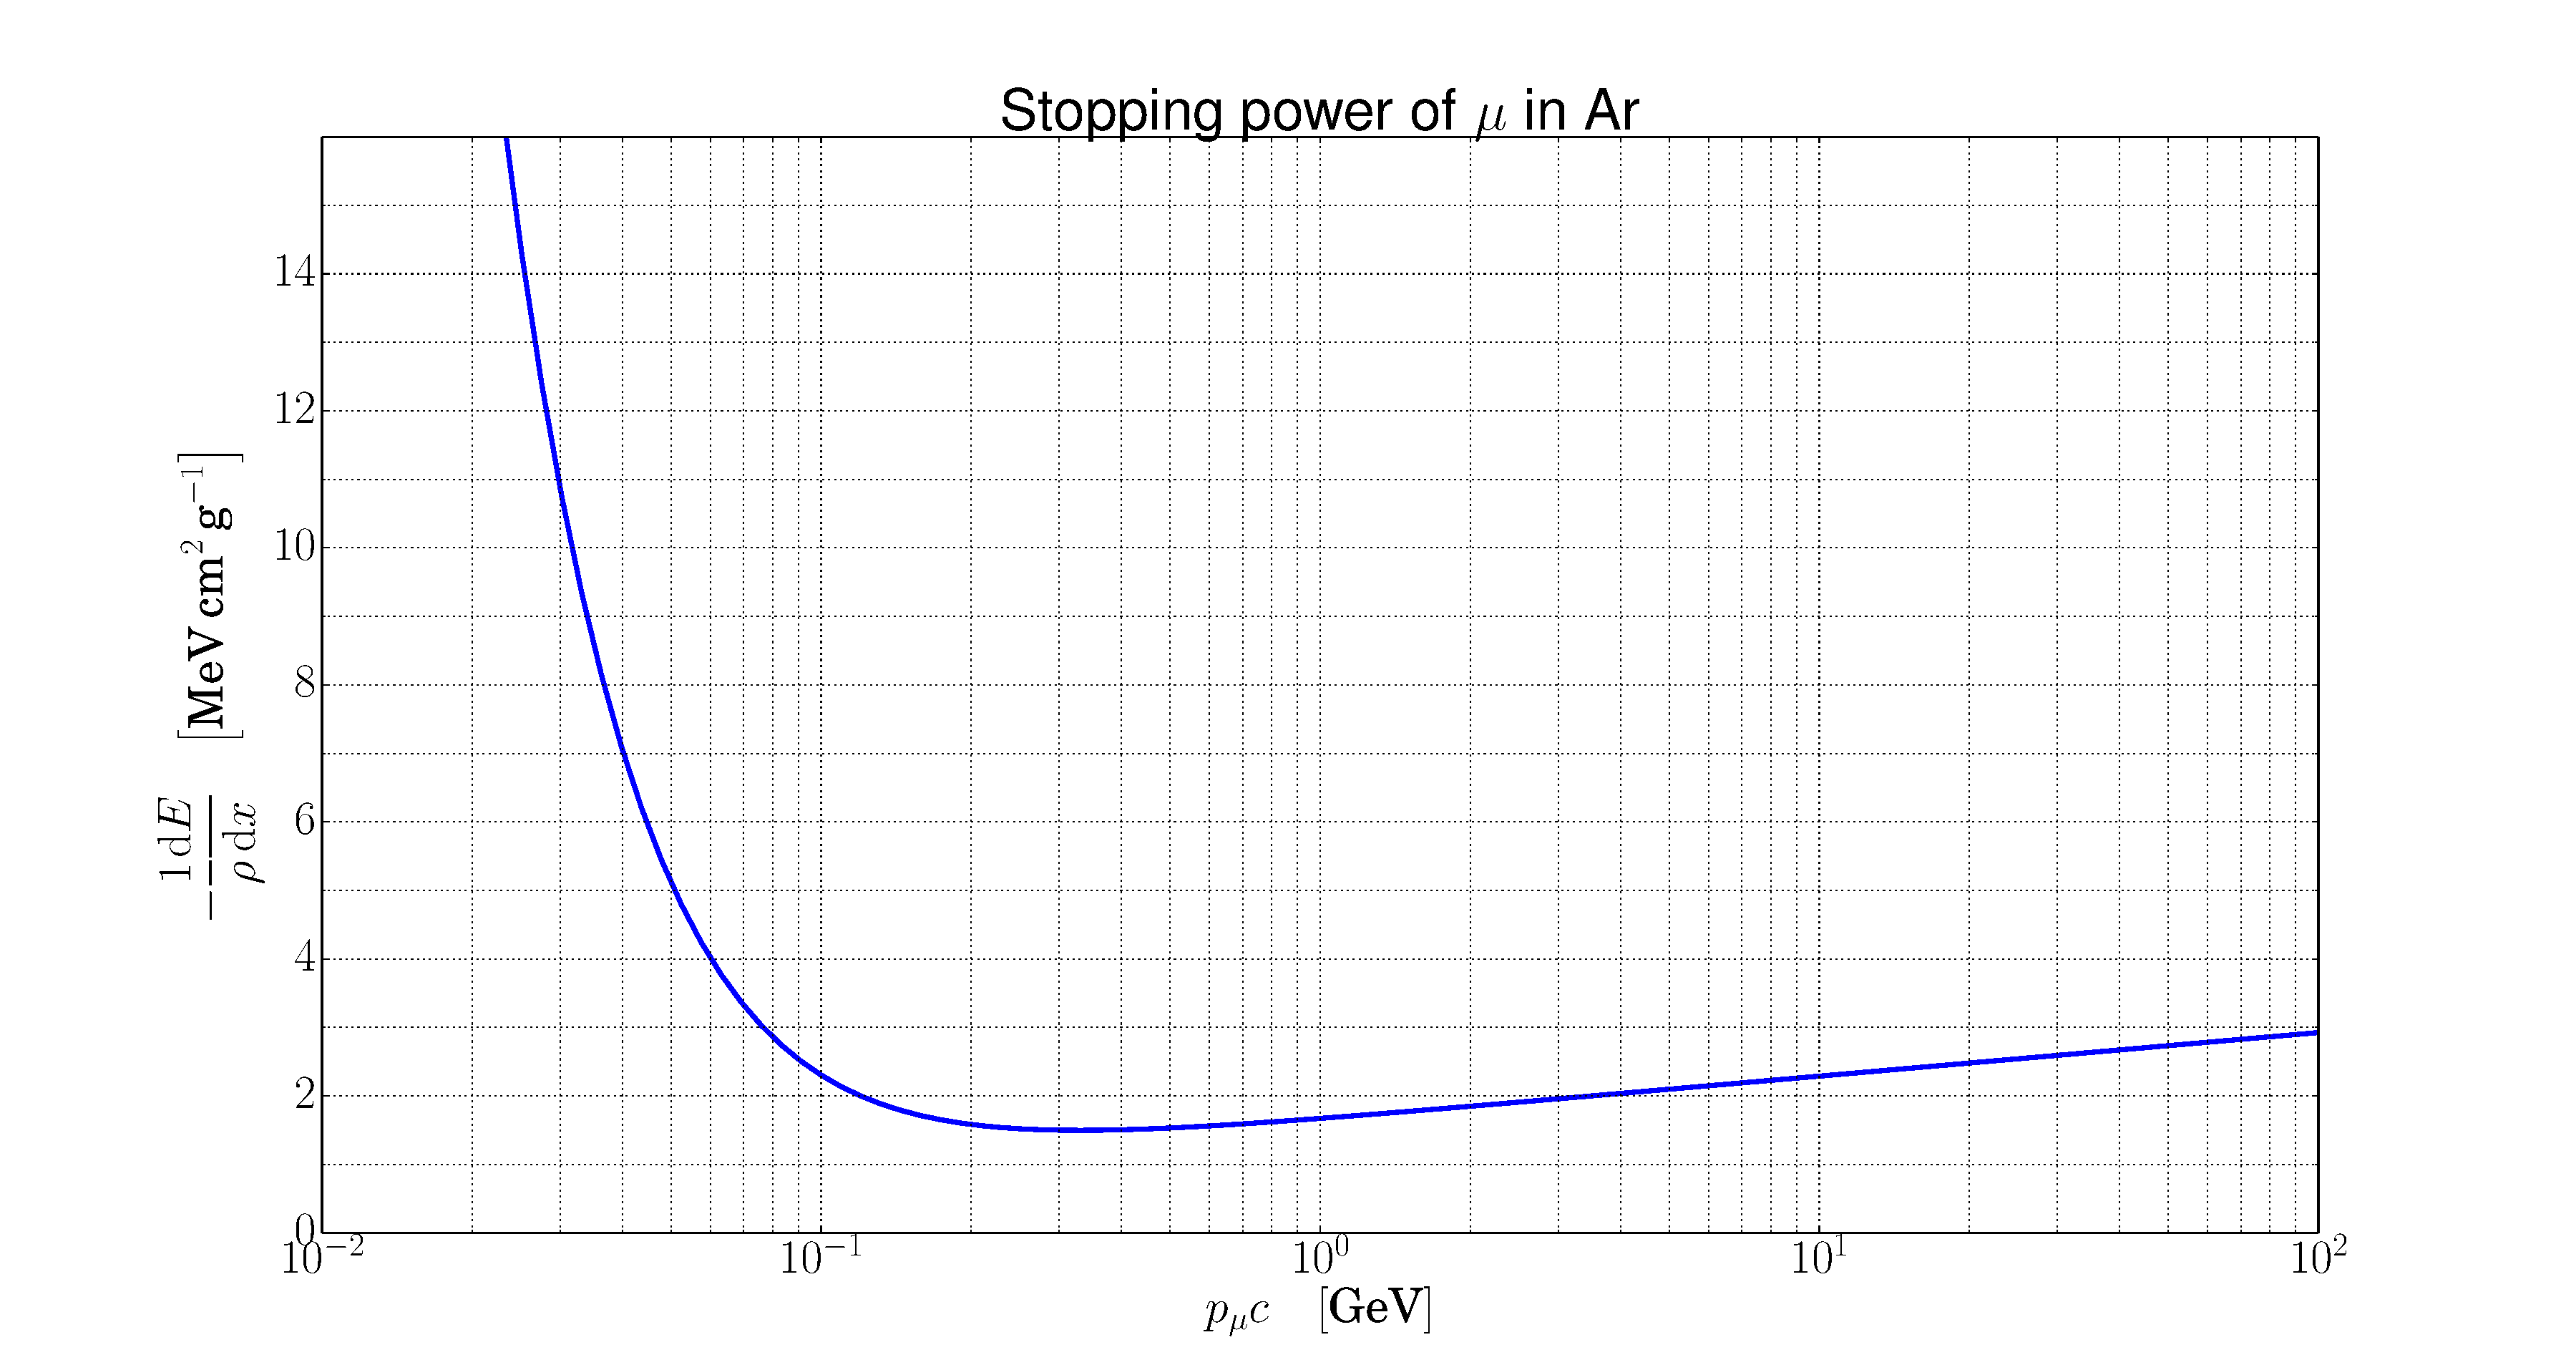
\includegraphics[width=\textwidth]{nu-detection/bethe-bloch}
	\caption{Bethe-Bloch stopping power of $\mu$ in \ce{Ar}}
	\todo[inline]{check}
	\label{fig:nu-detection_bethe-bloch}
\end{figure}

Figure~\ref{fig:nu-detection_bethe-bloch} shows the mass stopping power of $\mu$ in \ce{Fe} neglecting the $\frac{\delta}{2}$ term.
As can be seen, there is a broad minimum which is characteristic of the Bethe-Bloch formula.
Particles in this momentum range are called minimum ionising particles (MIPs).
They are important for detectors because this energy loss is a measure for the required energy resolution of a detector.
As mentioned above, the mass stopping power only loosely depends on the absorber material and therefore, its minimum is
\begin{IEEEeqnarray}{rCl}
	\eval{- \frac{1}{\rho} \dv{E}{x}}_{\m{min}} & \approx & \SI{2}{\mega\electronvolt\centi\meter\squared\per\gram}
\end{IEEEeqnarray}
for singly charged incident particles on most (light) absorbers.
To the left of the minimum is the \emph{Bragg peak} which is especially important for radiation therapy with heavy charged particles (e.g.\ protons).
The Bragg peak falls off with a strong $\frac{1}{\beta ^ 2}$ dependence.
After the minimum, the stopping power rises again with a logarithmic dependence on $\beta$ and the mean excitation energy of the absorber $I$.
The reason for this so called \emph{logarithmic rise} is the extension of the transverse electric field of the incident particle in the relativistic regime.
Due to increasing shielding of the transverse electric field by the shell electrons of the absorber materials, taken into account by the $\frac{\delta}{2}$ term, the rise is only asymptotic.
For electrons and positrons, Equation~\eqref{eq:nu-detection_bethe-bloch} does not hold because their mass is equal to the mass of the atomic electrons of the absorber.
The stopping power changes further for electrons because the incident particle cannot be distinguished form its collision partner in that case.
On the other hand, a positron will be annihilated upon stop by an electron which needs to be taken into account as well.
The equivalent of Equation~\eqref{eq:nu-detection_bethe-bloch} for $e^{\pm}$ can be found in~\cite{grupen}.

At high velocities, further effects come into play.
\emph{Bremsstrahlung} describes the radiation energy loss of a fast charged particle in the Coulomb field of the absorber nuclei.
It can be described by
\begin{IEEEeqnarray}{rCl}
	- \frac{1}{\rho}\dv{E}{x} & = & \frac{E}{X_{\m{0}}}
	\label{eq:nu-detection_bremsstrahlung}
\end{IEEEeqnarray}
where
\begin{IEEEeqnarray}{rCl}
	X_{\m{0}} & = & \frac{A}{4 \alpha N_A Z \qty(Z + 1) \qty(\frac{1}{4 \pi \varepsilon_{\m{0}}} \frac{\si{\elementarycharge} ^ 2}{m c ^ 2}) ^ 2 \ln(183 Z ^ {- \frac{1}{3}})}
	\label{eq:nu-detection_radiationlength}
\end{IEEEeqnarray}
is the \emph{radiation length} of the absorber material using
\begin{itemize}
	\item[$\alpha$] $\approx \frac{1}{137}$ the fine-structure constant and
	\item[$m$] the mass of the incident particle.
\end{itemize}
Again, the energy loss is proportional to the density of the absorber and for convenience, divided by the latter.
Bremsstrahlung is emitted in interactions of the incident particle with the absorber nuclei ($\propto Z ^ 2$) as well as with the atomic electrons of the absorber ($\propto Z$).
By neglecting the latter, one obtains the important relation
\begin{IEEEeqnarray}{rCl}
	X_0 ^ {- 1} & \propto & Z ^ 2
\end{IEEEeqnarray}
as opposed to the $\propto Z$ dependence of the Bethe-Bloch formula.
Equation~\eqref{eq:nu-detection_bremsstrahlung} also holds for electrons as long as $E \gg \frac{m_{\m{e}} c ^ 2}{\alpha Z ^ {\frac{1}{3}}}$.
Furthermore, looking at the dependence on the mass of the incident particle, one finds
\begin{IEEEeqnarray}{rCl}
	X_0 & \propto & m ^ 2
\end{IEEEeqnarray}
using Equation~\eqref{eq:nu-detection_radiationlength}.
Therefore, the radiation length of an absorber material is usually given for electrons and the relation
\begin{IEEEeqnarray}{rCl}
	X_0 & = & X_0^{\m{e}} \frac{m ^ 2}{m_{\m{e}} ^ 2}
\end{IEEEeqnarray}
can be used to get the radiation length for any charged particle of mass $m$.
Radiation losses play a significant role only at energies much higher than the energy of MIPs.
Using Equations~\eqref{eq:nu-detection_bethe-bloch} and~\eqref{eq:nu-detection_bremsstrahlung}, one can define a \emph{critical energy} $E_{\m{c}}$ by
\begin{IEEEeqnarray}{rCl}
	\eval{\dv{E}{x}_{\m{ion}}}_{E_{\m{c}}} & = & \eval{\dv{E}{x}_{\m{brems}}}_{E_{\m{c}}}
	\label{eq:nu-detection_ec}
\end{IEEEeqnarray}
at which radiation losses take over from ionisation losses.
Similar to the radiation length, the critical energy is proportional to $m ^ 2$.
Thus, it is most important for electrons while for other particles it becomes significant only at very high energies.
If we take the example of an iron absorber again for instance, we get $E_c^{\m{e}} = \SI{20.7}{\mega\electronvolt}$ and $E_c^{\mu} = \SI{890}{\giga\electronvolt}$.

At high energies, there are additional types of radiation loss taking place, for instance direct electron-pair production and photonuclear interactions.
They shall not be described here.
Instead, only their $\propto E$ relation similar to bremsstrahlung losses shall be mentioned.
A description of those effects can be found in~\cite{grupen}.

In addition to the processes described above, charged particles traversing matter also undergo scattering in the Coulomb field of the nuclei of the traversed medium.
Accordingly, this process is called \emph{multiple Coulomb scattering} or MCS.
The root mean square of the \emph{scattering-angle distribution}
\begin{IEEEeqnarray}{rCl}
	\Theta_{\m{RMS}} & = & \frac{\SI{13.6}{\mega\electronvolt}}{\beta c p} z \sqrt{\frac{2 x}{X_{\m{0}}}} \qty[1 + 0.038 \ln(\frac{x}{X_{\m{0}}})]
	\label{eq:nu-detection_highland}
\end{IEEEeqnarray}
is defined by the momentum $p$, velocity $\beta c$ and charge $z$ of the scattered particle, and the thickness of the scattering medium $\frac{x}{X_{\m{0}}}$ in radiation lengths.
The distinct momentum dependence of this so-called \emph{Highland formula} can be used to reconstruct the momentum of the incident particle provided the angular resolution of the detector is fine enough.

Concerning the interactions of charged particles with matter, there is one important note regarding detectors.
While charge produced in interactions (i.e.\ ionisation) can be detected directly, light (i.e.\ excitation photons and photon radiation) first needs to be converted to charge to be detected.
This conversion from light to electric charge is the topic of the next section.

Photons can interact with matter in different ways.
In particular, they can be converted to charge which can be detected.
The three most important interactions converting photons to charge shall be outlined in this section.
All of them have in common that they attenuate photon beams exponentially according to
\begin{IEEEeqnarray}{rCl}
	I & = & I_0 \m{e} ^ {- \mu x}
\end{IEEEeqnarray}
where $I_0$ and $I$ is the intensity before and after passing the absorber, respectively.
The thickness of the absorber is given by $x$ and
\begin{IEEEeqnarray}{rCl}
	\mu & = & \frac{N_A}{A} \sum_i \sigma_i
	\label{eq:nu-detection_mass-att-coeff}
\end{IEEEeqnarray}
is the \emph{mass attenuation coefficient} defined by the sum of the cross sections $\sigma_i$ of the different interaction processes.

At low energies (ionisation energy $\le E_{\gamma} \le \SI{100}{\kilo\electronvolt}$), photons primarily undergo conversion to charge by the \emph{photoelectric effect}.
The photon is absorbed by an atom of the absorber which in turn is ionised and thus ejects one of its shell electrons.
The cross section is given by
\begin{IEEEeqnarray}{rCl}
	\sigma_{\m{photo}} = \qty(\frac{32}{\epsilon ^ 7}) ^ \frac{1}{2} \alpha ^ 4 Z ^ 5 \sigma_{\m{Th}}^{\m{e}}
\end{IEEEeqnarray}
where
\begin{itemize}
	\item[$\epsilon$] $= \frac{E_{\m{\gamma}}}{m_{\m{e}} c ^ 2}$ is the reduced photon energy and
	\item[$\sigma_{\m{Th}}^{\m{e}}$] $= \frac{8}{3} \pi r_{\m{e}} ^ 2 = \SI{6.65e-25}{\centi\meter\squared}$ is the \emph{Thomson cross section} for elastic scattering of photons on electrons.
\end{itemize}

For energies $\approx \SI{1}{\mega\electronvolt}$, \emph{Compton scattering} dominates the interaction of photons with matter.
Thereby, the photon is not absorbed by the atom but just scatters off one of its shell electrons with the cross section
\begin{IEEEeqnarray}{rCl}
	\sigma_{\m{c}} & = & 2 \pi r_{\m{e}} ^ 2 Z \left\{\qty[\frac{1 + \epsilon}{\epsilon ^ 2}] \qty[\frac{2 \qty(1 + \epsilon)}{1 + 2 \epsilon} - \frac{1}{\epsilon} \ln(1 + 2 \epsilon)]\right.\\
	& & \left. + \frac{1}{2 \epsilon} \ln(1 + 2 \epsilon) - \frac{1 + 3 \epsilon}{\qty(1 + 2 \epsilon) ^ 2}\right\}
\end{IEEEeqnarray}
obtained from the Klein-Nishina formula.
As only part of the photon's energy is absorbed while the rest is scattered, it makes sense to divide this cross section into a scattering cross section
\begin{IEEEeqnarray}{rCl}
	\sigma_{\m{cs}} & = & \frac{E_{\gamma}'}{E_{\gamma}}
\end{IEEEeqnarray}
and an absorption cross section
\begin{IEEEeqnarray}{rCl}
	\sigma_{\m{ca}} & = & \sigma_{\m{c}} - \sigma_{\m{cs}}
	\label{eq:nu-detection_sigma-compton}
\end{IEEEeqnarray}
where $E_{\gamma}$ and $E_{\gamma}'$ is the energy of the photon before and after scattering, respectively.

At $E_{\gamma} \ge 2 m_{\m{e}} c ^ 2$, photons are capable of producing pairs of $e^+ e^-$.
Because of momentum conservation, this process can only happen in the coulomb field of a so called spectator particle.
As pair-production in the field of an electron is strongly suppressed, the spectator is usually a nucleus of the absorber material.
Therefore, the cross section of pair-production depends on the shielding of the coulomb field by the shell electrons and thus on the proximity to the nucleus.
Eventually, this results in an energy dependence.
For $1 \ll \epsilon < \frac{1}{\alpha Z ^ {\frac{1}{3}}}$, the cross section is given by
\begin{IEEEeqnarray}{rCl}
	\sigma_{\m{pair}} & = & 4 \alpha r_{\m{e}} ^ 2 Z ^ 2 \qty(\frac{7}{9} \ln 2 \epsilon - \frac{109}{54})
\end{IEEEeqnarray}
and for $\epsilon \gg \frac{1}{\alpha Z ^ {\frac{1}{3}}}$, the cross section is
\begin{IEEEeqnarray}{rCl}
	\sigma_{\m{pair}} & = & 4 \alpha r_{\m{e}} ^ 2 Z ^ 2 \qty[\frac{7}{9} \ln(\frac{183}{Z ^ {\frac{1}{3}}}) - \frac{1}{54}] \m{.}
\end{IEEEeqnarray}

As mentioned above, for Compton scattering, two different cross sections are defined, $\sigma_{\m{cs}}$ for the scattered energy and $\sigma_{\m{ca}}$ for the absorbed energy.
Consequentially, there are also different definitions of the coefficient $\mu$ in Equation~\eqref{eq:nu-detection_mass-att-coeff}.
Replacing the total Compton cross section $\sigma_{\m{c}}$ by $\sigma_{\m{ca}}$ from Equation~\eqref{eq:nu-detection_sigma-compton}, one gets the \emph{mass absorption coefficient} $\mu_{\m{a}}$, only taking into account photon absorption processes.
While $\mu$ is more precisely called the \emph{total mass attenuation coefficient}.

An interesting effect takes place for $e^{\pm}$ traversing material at energies higher than the critical energy $E_{\m{c}}$ defined by Equation~\eqref{eq:nu-detection_ec}.
In this regime, the energy loss is dominated by bremsstrahlung for $e^{\pm}$ and by pair production for $\gamma$.
This leads to an \emph{electromagnetic (EM) cascade} or \emph{shower} where $e^{\pm}$ and $\gamma$ produce each other alternately in a self-sustaining process.
The mean free path of a $\gamma$ before pair production
\begin{IEEEeqnarray}{rCl}
	\lambda_{\m{prod}} & = & \frac{9}{7}X_{\m{0}}
\end{IEEEeqnarray}
is very close to the mean free path of an $e^{\pm}$ before bremsstrahlung, the radiation length $X_{\m{0}}$.
Therefore, the number of particles participating in the shower doubles roughly every radiation length resulting in an exponential growth.
When the average energy per paticle drops below the critical energy, ionisation losses begin to dominate over radiative losses for $e^{\pm}$ and Compton and photoelectric effect over pair production for $\gamma$.
At this point, the shower reaches its maximum and
\begin{IEEEeqnarray}{rCl}
	t_{\m{max}} & = & \frac{\ln(\frac{E_{\m{0}}}{E_{\m{c}}})}{\ln(2)}
\end{IEEEeqnarray}
is its longitudinal extent in radiation lengths.
The \emph{Molière radius}
\begin{IEEEeqnarray}{rCl}
	R_{\m{M}} & = & \frac{\SI{21}{\mega\electronvolt}}{E_{\m{c}}} X_{\m{0}}
\end{IEEEeqnarray}
is the transversal extent of the shower divided by the the material density.
Both $t_{\m{max}}$ and $R_{\m{M}}$ are important benchmarks for the dimensioning of electromagnetic calorimeters.
Naturally, a $\gamma$ in the energy range where pair production dominates will produce a shower as well.
On the other hand, also $\mu^{\pm}$ can start electromagnetic cascades, if there energy is high enough to produce bremsstrahlung.

Similarly, hadrons interacting with matter via the strong force can produce cascades as well.
As opposed to the electromagnetic showers governed only by $e^{\pm}$ and $\gamma$, the hadronic process is much more complex because many different secondary particle can be involved.
Hadrons start to shower because they mainly interact inelastically with matter, producing secondary strongly interacting particles.
That is why the hadronic cross-section
\begin{IEEEeqnarray}{rCl}
	\sigma_{\m{total}} & = & \sigma_{\m{elastic}} + \sigma_{\m{inel}}
\end{IEEEeqnarray}
is usually split.
From $\sigma_{\m{inel}}$, one can derive the \emph{interaction length}
\begin{IEEEeqnarray}{rCl}
	\lambda_{\m{I}} & = & \frac{A}{N_{\m{A}} \rho \sigma_{\m{inel}}}
\end{IEEEeqnarray}
which describes the absorption of hadrons in matter according to
\begin{IEEEeqnarray}{rCl}
	N & = & N_{\m{0}} e ^ {- \frac{x}{\lambda_{\m{I}}}}
\end{IEEEeqnarray}
with the initial number of hadrons $N_{\m{0}}$ and number of hadrons $N$ after a distance $x$ of absorber material.
For absorbers with $Z \geq 6$, the interaction length is much larger than the radiation length $X_{\m{0}}$ meaning that hadronic calorimeters usually need to be much larger than their electromagnetic counterparts.